\section{Literature review}

\todo{Insert literature review as a table}

\subsection{The modern approach}
As it can be seen from the preceding literature review, most robotic systems'
operation can be modeled by the commonly known \emph{Sense, Plan, Act}
paradigm:

\todo{Add custom act, sense, plan paradigm picture}
\begin{figure}[h]
	\centering
	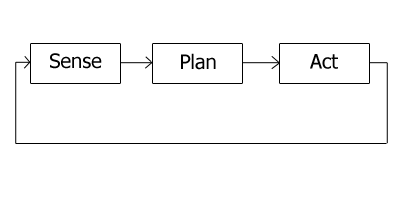
\includegraphics[width=0.4\textwidth]{figure/robotic_paradigm.png}
	\caption{The Sense, Plan, Act robotic paradigm.}
	\label{fig:robotic_paradigm}
\end{figure}

\begin{itemize}
	\item{\textbf{Sense}}: gather information using sensors (camera, IMU, sonar...).
	\item{\textbf{Plan}}: create a world model using all the information, and plan
		the next move.
	\item{\textbf{Act}}: carry out the actions that the plan calls for.
\end{itemize}

~\\
This thesis will be focused mainly on the sensing of the drone control, and
more precisely using deep learning and computer graphics. However, an important
part of the trajectory planning directly follows the sensing phase, therefore
those two first phases of the control loop can be included in the scope of the
project.

To this day, most drones in the robotic research field are running \emph{Robot
Operating System} (ROS), \todo{Add citation} which is a set of ``libraries and
tools to help software developers create robot applications''. It allows to
independently run programs as ``nodes'', which can communicate with each other
using a principle of ``subscription'' and ``publication`` on easily definable
topics, as represented on Figure~\ref{fig:ros-topics}.

\begin{figure}[h]
	\centering
	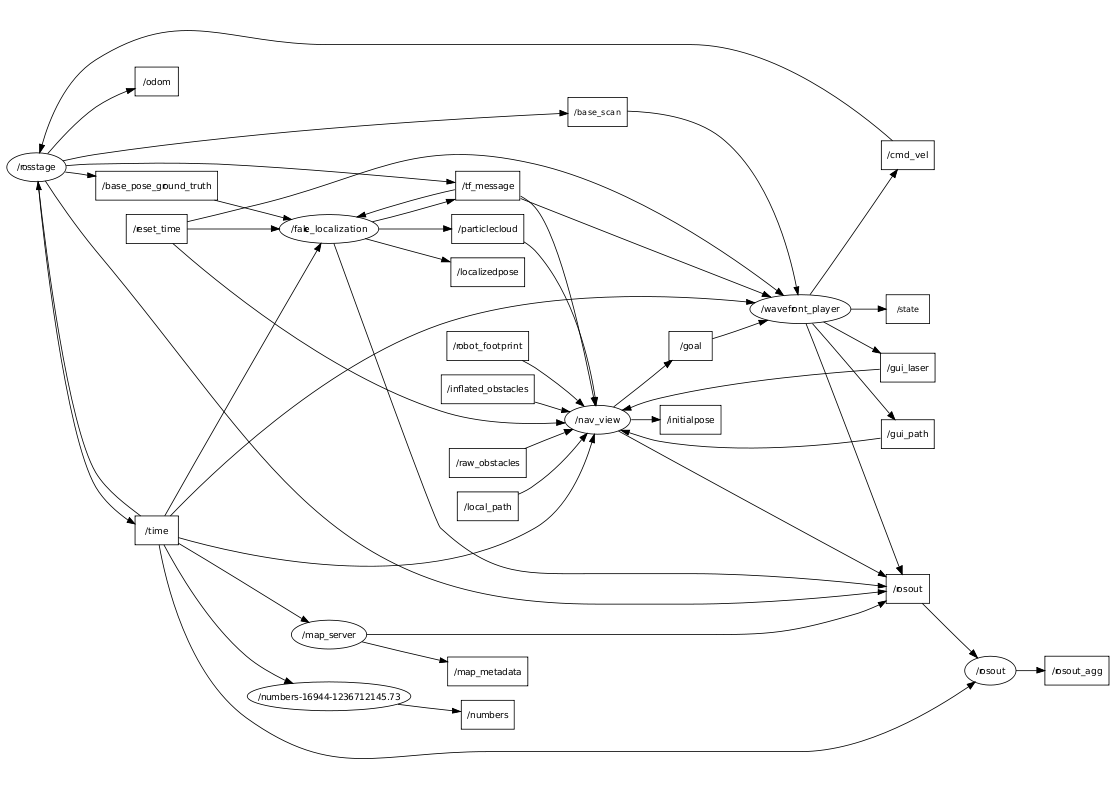
\includegraphics[width=0.7\textwidth]{figure/ros_topics.png}
	\caption{The ROS topics graph showing inter-node communications for this
	project.}
	\label{fig:ros-topics}
\end{figure}

ROS makes the transition between the simulated environment and the real world
seamless, because it can be installed on most Linux systems, and adds a layer
of abstraction between the hardware and the software, by distributing packages
built by the community.\\

The implementation of the computer vision algorithms will be constrained within
ROS, and cooperate with the different control components, in an effective
modular manner.\\

\todo{Talk about why CNNs are used more and more in drone racing, and basically
why it is the chosen approach, which leads to tackling the dataset generation
problem.}


As deep learning has known an exponential growth during the past decade,
computer vision applications tend to exploit the power of convolutional neural
networks more and more. Thanks to their impressive performance in specific
problem solving, CNNs are becoming the main choice for tasks such as: object
detection, object segmentation, object recognition, object tracking,
\emph{etc}\ldots

In drone racing, the latest works, which are often the best performing, tend to
employ CNNs for the sensing part, or even as an all-in-one solution. It is a
reasonable choice mainly because neural networks are observed to offer
robustness and accuracy, to the cost of computational power. They can be hard
to train, given their sporadic nature, but it is often a very good alternative
to developing a custom algorithm which can take a lot of time and does not
guarantee consistent results, in different lighting conditions for instance.

On that note, the chosen method for solving the drone racing challenge is
using a convolutional neural network, coupled with a simple state-machine 
using a PID controller to steer the drone.
